%math macros; figure out where these belong.
\newcommand{\ind}{\stackrel{ind.}{\sim}}
\newcommand{\op}{\operatorname}
\newcommand{\code}{\texttt}

\section{Introduction}
We consider the model given by $Y_{gi}|x_i \ind F(\theta_{g}| x_i)$, $g=1,\ldots,G$, $i=1,\ldots,N$ with $G\gg N$ and the quantities of interest are functions of $\theta_g$. In this setting, there is potential benefit to borrow information across group level, $g$, to reduce variance. A common approach is to assume that the $\theta_g$ are independent, identically distributed according to some probability distribution, $\mathcal{P}$, belonging to a parametric family of distributions. Under this framework, $\mathcal{P}$ can then be estimated allowing for conditional inference, or a prior distribution can be given on its parameters allowing for fully Bayesian inference. While this approach can be useful in practice, the influence of the choice of a particular parametric family can be considerable. This choice is often not reflective of a priori information, but rather due to convention or convenience. THe choice of a `nonparametric prior', or a prior distribution over the set of probability distributions in $\mathbb{R}^p$, avoids making parameteric assumptions about $\mathcal{P}$. The most widely used such prior distribution in the literature of Bayesian nonparametrics is the Dirichlet process (DP).

Much effort has gone into researching methods for analyzing gene expression. Some of the most successful have been made publically available as R packages \cite{edger2010},\cite{deseq2014}. These methods attempt to account for the mean-variance trend, which can vary from data set to data set. Similarly, plots of empirical estimates of $\beta_g$, coefficients of regression on a log scale, suggest complex structures of dependency among some components of $\beta_g$. These show distributional shapes -- features such as mulitmodality, spikes and heavy tails -- which are not easily characterized by a parametric distribution. These observations seem to suggest two things: a) a joint model, $(\beta_g, \sigma^2_g) \ind \mathcal{P}$, should be useful, by providing a means for regularizing inference that accounts for dependence between components, and b) the prior distribution for $\mathcal{P}$ should spread prior mass over a large distributional space.

A number of Gibbs sampling algorithms for MCMC have been proposed, based on a marginalization over the random measure $\mathcal{P}$ \citep{neal2000}. Variations of this have shown to be effective in practice. However, for large $G$, these algorithms are not computationally tractable as they require one-at-a-time updating of the cluster assignment for each $g$ conditioning on all $g'\neq g$. The ``stick-breaking" representation of the DP, due to \citet{sethuraman}, provides a way to explicitly sample $\mathcal{P}$. By conditioning on $\mathcal{P}$, the assignment of clusters can be done in parallel due to conditional independence. \citet{suchard} proposed algorithms for such ``massive" mixture models that target graphics processing units (GPUs), which use the inherent parallel processing power to acheive large speed-ups in computation time. In this paper we describe an implementation of the approach outlined by \citet{suchard}, and apply it to gene expression data.

Section \ref{sec:model} presents a hierarchical regression model for gene expression with truncated Dirichlet process prior. The full posterior distribution is given in subsection \ref{subsec:posterior}. Section \ref{sec:computation} offers general remarks regarding the implementation strategy. Subsections \ref{subsec:upsweep} and \ref{subsec:downsweep} provide some introductory material regarding parallel algorithms. The rest of this section describes the libraries and tools which were useful in developing our application. Section \ref{sec:implement} describes the details of our implementation, concentrating on the steps for the Gibbs sampler, which are at the core of our method. In subsection \ref{subsec:output} we consider how we cope with the memory bottleneck, which prevents storing most MCMC samples. Section \ref{sec:timing} presents a study of the rate of mixing for different sized data sets and sampler settings. In the final section, we consider some extensions...
% In summary, to avoid sensitivity to the prior distribution on $\mathcal{P}$, we propose to model it as a truncated Dirichlet process. Advances in computers have seen a rapid increase in the use of Markov Chain Monte Carlo (MCMC) methods for fitting sophisticated statistical models. Because such methods rely on thousands or even millions of simluated draws generated one after another, fast computing is critical to making them computationally feasible. Nonparametric Bayesian methods are no different in this regard, but when the size of the data set gets moderately large, the computational effort required per draw can be enormous as the number of parameters grows with the sample size. Graphics processing units (GPUs) have potential in this area, provided that most of the work can be divided into many parallel tasks which operate on different pieces of memory. By exploiting conditional independence in the model and making use of parallelized algorithms, we demonstrate the feasibility of nonparametric Bayesian modeling in the ``big data" setting of gene expression data.

\section{Model}
\label{sec:model}
Let $Y_{gci}$ represent the observed expression (possibly after transformation) for gene $g$, condition $c$, replicate $i$. Let $x_{ci}^\top$ be the row of the design matrix $X$ corresponding to replicate $i$ with condition $c$. We will use the upper case letters $G$, $C$ to denote the number of genes, and conditions and let $N$ denote the total number of samples. In addition, we accomodate possible quality weights, $w_{gci}$.  Note that one may wish to control for other experimental or technical factors, represented as columns in the design matrix, so that $x_{ci} \neq x_{cj}$ for $i \neq j$. However, we will assume that $p$,  the number of columns in $X$, is less that $N$. For the observed data, we assume the model
\begin{equation}
Y_{gci} \sim \op{N} \left( x_{ci}^\top \beta_g, \frac{\sigma^2_g}{w_{gci}} \right).
\end{equation}
Next, we propose to model jointly

\begin{equation}
\left(\beta_g^\top,\sigma^2_g\right) \ind \mathcal{P},
\end{equation}
where we specify a Dirichlet process prior

\begin{equation}
\mathcal{P} \sim \op{DP}(\alpha Q).
\end{equation}

This prior, due to \citet{ferguson}, is a distribution over probability distributions, such that for any finite disjoint partition $\{A_i\}_{i>=1}^n$ on $\mathbb{R}^p$, $\mathcal{P}$ is a random measure such that the joint distribution $\left(\mathcal{P}(A_1),\ldots,\mathcal{P}(A_n)\right) \sim \op{Dir}\left(\alpha Q(A_1),\ldots,\alpha Q(A_n)\right).$ The Dirichlet process has two parameters: $Q$, the base measure, represents a prior guess at the distribution. $\alpha$, the concentration parameter expresses the degree to which $\mathcal{P}$ will agree with $Q$ on any set $A$. This follows from the definition given above and known properties of the Dirichlet distribution, i.e., $\op{E}\left(\mathcal{P}(A)\right)=Q(A)$, and $\op{V}\left(\mathcal{P}(A)\right)=\frac{Q(A)(1 - Q(A)}{\alpha + 1}$, showing that $\mathcal{P}(A) \stackrel{p}{\rightarrow} Q(A)$ as $\alpha \rightarrow \infty$ for any set $A$. 

As shown by \citet{sethuraman}, it follows from this definition that $\mathcal{P}$ is almost surely discrete and realizations of $\mathcal{P}$ can be produced by the following stick-breaking construction:

Let 
\begin{equation}
\mathcal{P} =\sum_{k=1}^\infty \pi_k \delta_{\left(\tilde{\beta}_k^\top ,\tilde{\sigma}^2_k\right)}.
\end{equation}
Here $\delta_{(.)}$ is the Dirac delta function. The ``atoms" distributed according to $Q$, specified by the product measure

\begin{equation}
\tilde{\beta}_k \sim \op{N}(m_\beta, C_\beta),\quad \tilde{\sigma}^2_k \sim \op{IG}(a_{\sigma^2}, b_{\sigma^2}).
\end{equation}

We choose values of $m_\beta,\,C_\beta,\,a_{\sigma^2},\,b_{\sigma^2}$ to put mass on reasonable values of $\left(\beta_g^\top,\sigma^2_g\right)$. This is important for the efficiency of our MCMC algorithm.

The mixture weights, $\pi_k$,  follow a stick-breaking process \cite{sethuraman}. Using the reparameterization,

\begin{equation}
\nu_k = \frac{\pi_k}{1 - \sum_{l=1}^{k-1} \pi_l},
\end{equation}

$\nu_k$ representing a proportion of the total probability remaining after $k-1$ breaks, we assume
\begin{equation}
\nu_k \ind \op{Beta}(1, \alpha).
\end{equation}

Note that $\sum_{k=1}^K \pi_k \rightarrow 1$ as $K\rightarrow \infty$. Additionally, this assumption induces a decreasing stochastic ordering of the weights. The parameter $\alpha$ plays an important role in the model, since it helps to determine how quickly the successive elements of $\pi$ decay, i.e. the number of clusters selected by the model. For computational convenience, we choose the conditionally conjugate prior

\begin{equation}
\alpha \sim \op{Gamma}(a_\alpha,b_\alpha).
\end{equation}

This prior can be selected to express an a priori belief on the number of clusters, $K_{occ}$, in the data. \citet{escobar1994} give expression for the expected value of $K_{occ}$ given $\alpha$ and $G$ as,
\begin{equation}
\op{E}(K_{occ})=\sum_{g=1}^{G} \frac{\alpha}{\alpha + g - 1}.
\end{equation}
In that paper, the authors use a table of values derived from this formula to defend their proposal for a prior over values of $\alpha$ ranging from $G^{-1}$ to $G^{2}$, which admits values of $\op{E}(K_{occ})$ anywhere from 1 to $G$. Due to computational limitations (we require $K_{occ} \ll G$), and our prior belief, based on scientific evidence, that there are more than just a few clusters, we choose $a_\alpha=3$ and $b_\alpha=\frac{3}{G^{.5}}$ to express a prior that $\op{E}(K_{occ})$ is probably between $G^{.5}$ and $G^{.75}$ (see figure \ref{alphaprior}).

\begin{figure}
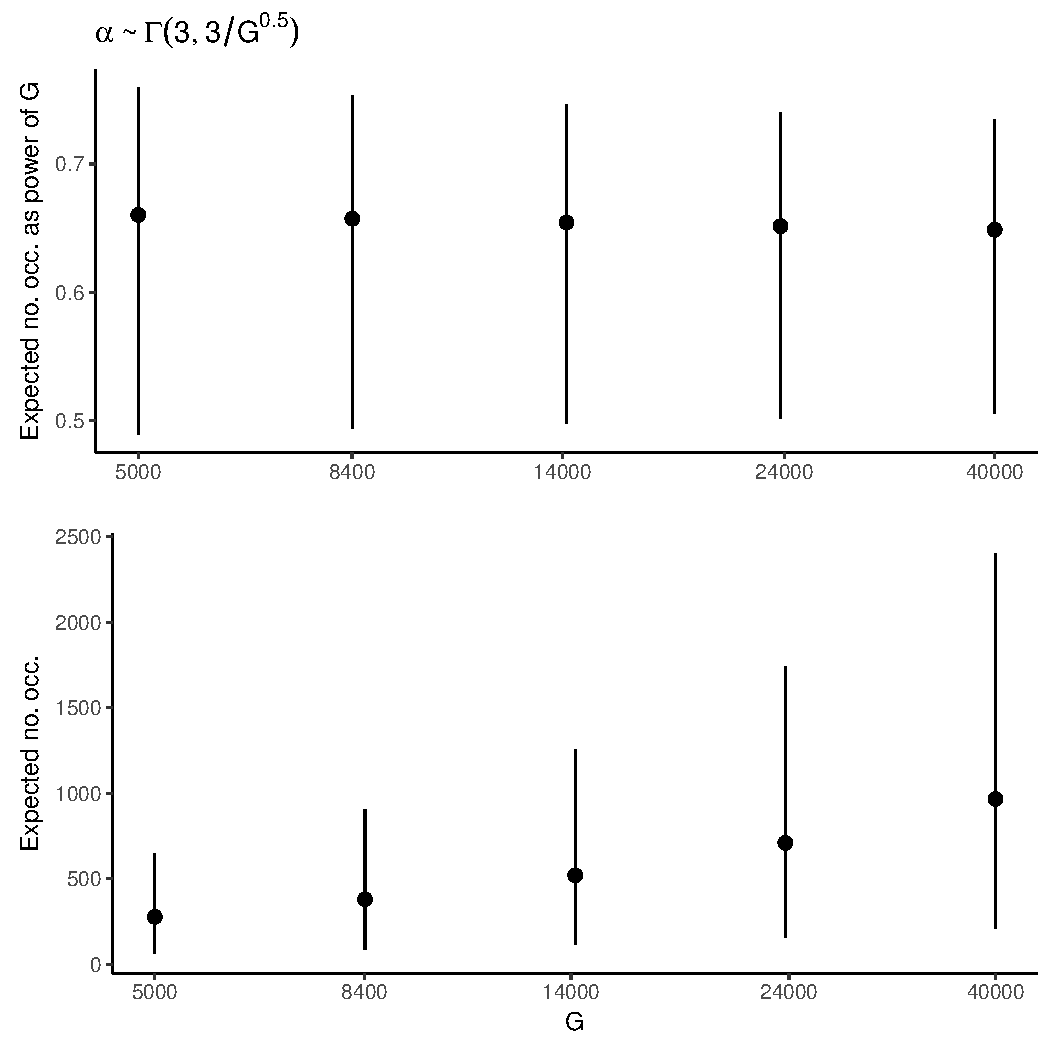
\includegraphics[width=.5\textwidth]{alphaprior}
\caption{The number of clusters determined by the model is influenced by the parameter $\alpha$, whose value determines the expected number of clusters prior to seeing the data. The figures above demonstrate the prior distribution of the prior expected number of clusters, $\op{E}(K_{occ})$ for datasets with various number of genes, $G$.}
\label{alphaprior}
\end{figure}

\subsection{Data augmentation and truncation}
\label{subsec:reparam}
To help construct a Gibbs sampler for this model, we use the ``augmented data" approach \cite{tanner}. Let $\zeta_g$ be a random variable taking values on the positive integers with prior distribution given by $Pr(\zeta_g=k)=\pi_k$. By conditioning on these allocation parameters, all $\tilde{\beta}_k$ are conditionally independent given $y$. Also, $\pi$ only depends on the data through $\zeta$.

We can acheive conditional independence among the $\zeta$ by approximating the unknown infinite mixture $\mathcal{P}$ by a truncated, finite mixture approximation to the Dirichlet process. $\mathcal{P}_K$. We do this by setting $\nu_K=1$, or equivalently, setting $\pi_K = 1 - \sum_{k<K} \pi_k$. This approximation was proposed by \citet{ishwaran2000}. The authors showed a method for selecting $K$ sufficiently large so as to make the difference between $\mathcal{P}$ and $\mathcal{P}_K$ arbitrarily small with respect $\mathcal{L}_1$ distance. 

In general, scientific questions will be restricted to those which can be formulated as sets of linear inequalities in $\beta_g$. 
%question: in genes with small counts, does this assumption lead to multimodality in posterior for beta_g?

\subsection{Posterior distribution}
\label{subsec:posterior}
Applying Bayes' theorem, the posterior distribution, up to a constant, is
\begin{equation*}
p(\beta,\sigma^2,\mathcal{P}|y) = p(\zeta, \tilde{\beta},\tilde{\sigma^2},\nu | y) \propto p(y|\tilde{\beta},\tilde{\sigma^2},\zeta) p(\zeta|\nu) p(\nu|\alpha)p(\tilde{\beta},\tilde{\sigma^2})
\end{equation*}
\begin{equation*}
= \prod_{g=1}^G \left\{ \op{N}(y_g;\,\beta_{\zeta_g},\sigma^2_{\zeta_g})\; \op{Cat}(\zeta_g;\, \pi(\nu)) \right\} \prod_{k=1}^K \left\{ \op{Be}(\nu_k;\, 1, \alpha)\; \op{N}(\tilde{\beta_k};\,\eta, \tau^2)\;\op{IG}(\tilde{\sigma}^2_k;\,\gamma,\lambda)\right\} \op{G}(\alpha;\Gamma,\Omega) 
\end{equation*}
The first equality follows from the  invariance to reparameterization of the posterior distribution, and the last equality follows from the product rule of conditionally independent random variables.

\section{Computation on the GPU}
\label{sec:computation}
\subsection{General Remarks}
Modern GPUs offer hundreds or thousands of cores that can all execute a program concurrently. This is a big advantage over multi-core CPUs which typically have fewer than ten processors. If one decides to implement a program using a GPU, there are contraints that they need to be aware of.
\begin{itemize}
\item
In the usual set-up, the main program in run on a CPU which turns over control periodically to the GPU to run specific tasks. These tasks, or ``kernels", follow the single instruction, multiple data (SIMD) paradigm. Each core on the GPU is assigned to work on a specific chunk of memory, but all cores execute the same program. Each instance of the program is called a ``thread". It is desirable to avoid branching logic in kernels, in part because the GPU cores are relatively slow, so branching can easily lead to high latency. The best results are obtained by having all threads proceed in lockstep.

\item
The GPU has its own memory system. Because copying memory from host (CPU) to device (GPU) and visa versa is slow, if possible, data input should be copied only once from the host CPU to GPU memory and when the task is completed, it should be copied once back only once to the CPU.

\item
When programming for the CPU, memory accesses tend to be fast. On the GPU, while the thread local memory is fast, its size is limited, and reading and writing from global memory is slow. Therefore, kernels need to limit both reads and memory allocation, or else the potential gain in speed due to parallelism will be lost due to memory bottlenecks.

\item
Threads are themselves organized into ``warps". When data is read from global memory, it reads not one address at a time, but in chunks to minimize overhead costs. To take advantage of this, consecutively indexed threads should use data from memory at consecutive addresses. When this happens, the reads are ``coalesced". If consecutive threads access addresses that are distant to one another, reads are not coalesced, which will make memory transfer inefficient, hence the program will tend to be slow.
\end{itemize}

\subsection{Routines}
\subsubsection{Reductions}
\label{subsec:reduce}
On the GPU, individual processors are slow, memory transfer is slow, and asynchronous tasks can result in many idle threads. In order to acheive speed-ups, algorithms must exploit parallelism and must do so in a way that respects the limitations of the hardware. A simple example is reduction. Given some data in memory, $x_1, x_2, \ldots, x_n$, and an \textit{associative} operator $\oplus$, the problem is to compute $x_1 \oplus x_2 \oplus \ldots \oplus x_n$. 

\begin{pseudocode}[ruled]{Reduce}{a}
\label{upsweep}
\COMMENT{Parallel reduction of $n=2^d$ elements (upsweep step of scan).}\\
\FOR i \GETS 1 \TO \log_2 n \DO \BEGIN
  \FOR j \GETS 1 \TO n \mbox{ in parallel }\DO \BEGIN
    \IF j \mbox{ mod } 2^i \DO \BEGIN
    a[j] \GETS a[j-2^{i-1}] + a[j];\\
    \END \END \END
\RETURN{a}
\end{pseudocode}

Assuming no constraint on the number of processors, algorithm \ref{upsweep} describes a GPU-friendly way to tackle this problem. In the first iteration of the outer loop, the inner loop keeps a maximal number of threads are busy with an identical task, requiring similar and parallel memory accesses, two reads and one write. While half of these threads become idle in subsequent loops, the active threads always write to the same place. In practice, since device memory is not flat, as was discussed in the previous subsection, an optimal implementation would make use of shared memory after the first read. Reading and writing from shared memory is much faster than from global memory and is accessible to all threads in a block.

% CUDA users who want to take advantage of GPU parallelism without concerning themselves with the optimization should be aware of the Thrust library \cite{thrust}. Thrust is based on the C++ Standard Template Library and provides both containers for handling allocation and deallocation of device memory as well as generic algorithms, such as \code{thrust::reduce}.


%\caption{Parallel reduction of $n=2^d$ elements (upsweep step of scan). Upon return, total is stored in $a[n]$.}

\subsubsection{Scans}
\citet{blelloch1990} described a general algorithm for computing $x_1,
x_1 \oplus x_2, \ldots, x_1 \oplus \ldots \oplus x_n$. This result is required at multiple points in our MCMC algorithm. An example is the calculation of cumulative probabilities in multinomial sampling. (In this case, the probabilities are on the log scale for stability, so that $\oplus=\log(e^{x_1}+e^{x_2})$.) The natural serial algorithm, $z_1 = x_1,\;z_2 = z_1 \otimes x_2,\dots$, is ill-suited to the GPU. Blelloch showed that there is an efficient parallel alternative. The simple case of an array with $2^d$ elements and $2^{d-1}$ processors consists of a parallel reduction (``upsweep"; algorithm \ref{upsweep}), followed by a downsweep (algorithm \ref{downsweep}. Given an input array $a$, the algorithm modifies the input with the result that each element contains the sum of all the previous elements in the original. In some cases this is the desired result; otherwise, the array is shifted to the right and the total from the upsweep is appended. In case that the number of threads is restricted, a solution is to divide the data up among the processors and perform a reduction on each subset. Next, a prescan can be performed on the processor totals, which are stored to memory. Finally, a series of scans can be performed on the subsets as desired, using the scanned processor totals as offsets \cite{blelloch1990}.
\begin{pseudocode}[ruled]{Prescan}{a}
\label{downsweep}
\COMMENT{Produce prescan of the original elements in $a$.}\\
a \GETS \CALL{Reduce}{a}\\
a[n] \GETS 0\\
\FOR i \GETS d \TO 1 \DO \BEGIN
  \FOR j \GETS 1 \TO n \mbox{ in parallel }\DO \BEGIN
    \IF j \mbox{ mod } 2^i = 2^{i-1} \DO \BEGIN
    tmp \GETS a[j];\\
    a[j] \GETS a[j + 2^{i-1}];\\
    a[j + 2^{i-1}] \GETS tmp \oplus a[j + 2^{i-1}];
    \END \END \END
\RETURN{a}
\end{pseudocode}


If $P$ processors are available
the time required to scan $n$ elements is on the order $O(n/P + \log_2P)$, versus $O(n)$ for the serial algorithm. This is the same as the parallel reduction.
% Parallel scans are implemented in Thrust, called with \code{inclusive\_scan} for a full scan and \code{exclusive\_scan} for a prescan.
%\subsubsection{Pseudo-random number generation}

% Parallel uniform and normal random number generation. For the (inverse) gamma draws, the method of \citet{simplegamma} is used, pairs of which can be transformed to produce beta draws.

%\subsubsection{Linear algebra}
%For computationally intensive tasks, such as matrix multiplication, much of the work can be done independently. Because much of the work requires repeated use of the same data, however, the optimal solution depends on both the hardware and the size of the problem. Fortunately, much of this work has already been done. Just as is the case in plain C, it is recommended to use APIs to optimized, documented libraries which are being developed and made available for GPUs.
% Many LAPACK/BLAS routines, including matrix multiplication, solving lower triangular matrix equations, matrix-vector multiplication and dot product.


\section{MCMC}
\label{sec:mcmc}
\subsection{Full conditionals}
\label{subsec:full-cond}
Our blocked Gibbs sampler is constructed as follows:
\begin{enumerate}
\item[Step 1:]
The allocation parameters, $\zeta_g$ are conditionally independent given $\pi, \beta, \sigma^2$ and the full conditional distribution is given by

\begin{equation}
\label{zetafull}
Pr(\zeta_g=k|\cdot) \propto \pi_k \op{N}(y_g;X\tilde{\beta}_k,\tilde{\sigma}_k^2 W_g),
\end{equation}
thus requiring multinomial sampling.

\item[Step 2:] Conditional on the allocation parameters, the full conditionals for $\tilde{\beta}_k$ and $\tilde{\sigma}^2_k$ are straightforward. Importantly, $\tilde{\beta}_k$ are conditionally independent and so are $\tilde{\sigma}^2_k$. However, for a given $k$, the full conditional for $\tilde{\beta}_k$ depends on $\tilde{\sigma}^2_k$, and visa versa. Hence, this represents a Gibbs-within-Gibbs.
  \begin{enumerate}
  \item[(a)] The full conditional for cluster location, $\tilde{\beta}_k$:
    \begin{equation}
      p(\tilde{\beta}_k|\cdot) \propto \prod_{g:\zeta_g=k} \op{N}(y_g;\,X\tilde{\beta}_k, \sigma^2_gW^{-1}_g)\,\op{N}(\tilde{\beta}_k; m, C)
    \end{equation}
    \begin{equation*}
      \implies p(\tilde{\beta}_k|\cdot) = \op{N}(\tilde{\beta}_k; \hat{m}_k,\, \hat{C}_k),
    \end{equation*}
    \begin{equation*}
    \mbox{ where }\hat{C}_k= \left( \sigma^{-2}_g\sum_{g:\zeta_g=k}
      X^\top W_g X + C^{-1} \right)^{-1}, \mbox{ and
    }\hat{m}_k=\hat{C}_k \left(\sum_{g:\zeta_g=k} X^\top W_g y_g +
      C^{-1}m \right).
    \end{equation*}
  \item[(b)] The full conditional for cluster variance, $\tilde{\sigma}_k^2$, is:
    \begin{equation}
      p(\tilde{\sigma}_k^2|\cdot) \propto \prod_{g:\zeta_g=k}
      \op{N}(y_g;\,X\tilde{\beta}_k, \sigma^2_gW^{-1}_g)
      \op{IG}(\tilde{\sigma}_k^2; a_{\sigma^2},b_{\sigma^2})
    \end{equation}
    \begin{equation*}
      \implies p(\tilde{\sigma}_k^2|\cdot) = \op{IG}(\hat{a}_k,\hat{b}_k), 
    \end{equation*}
    \begin{equation*}
      \mbox{ where }\hat{a}_k = a_{\sigma^2} + \frac{NM_k}{2},\mbox{ and }\hat{b}_k= b_{\sigma^2} + \sum_{g:\zeta_g=k}y_g^\top W_g y_g -2 \beta_g^\top X^\top W_g y_g  +\beta_g^\top X^\top W_g X \beta_g
    \end{equation*}

    Here $M_k$ is the number of $g$ for which $\zeta_g = k$. 
  \end{enumerate}
\item[Step 3:] The full conditional for $\nu_k,\,k=1,\ldots,K-1$ depends only on $M_k(\zeta)$. The full conditional is:

  \begin{equation}
    p(\nu_k) \propto \prod_{l \ge k} \prod_{g:\zeta_g=k} \pi_k \; \op{Be}(\nu_k; 1, \alpha) \propto \nu_k^{M_k + 1}(1-\nu_k)^{\sum_{l > k} M_l + \alpha} 
  \end{equation}
  \begin{equation*}
    \implies p(\nu_k)=\op{Be}(M_k + 1, \sum_{l>k}M_l + \alpha)
  \end{equation*}
\item[Step 4:]
  The concentration parameter, $\alpha$, has a conjugate gamma prior, and depends only on $\nu$. Its full conditional is:

  \begin{equation}
    p(\alpha|\cdot) \propto \prod_{k=1}^{K-1} \op{Be}(\nu_k;1, \alpha) \; \op{Ga}(\alpha;a_\alpha,b_\alpha)
\propto \alpha^{(K-1) + \Gamma - 1} \left(\prod_{k=1}^{K-1} (1-\nu_k)\right)^\alpha e^{-\Omega \alpha} 
  \end{equation}
  \begin{equation*}
    = \alpha^{(K-1) + a_\alpha - 1} e^{-(-\log \pi_K + b_\alpha) \alpha}
  \end{equation*}
  \begin{equation*}
    \implies p(\alpha|\cdot) = \op{Ga}(K + a_\alpha - 1, -\log \pi_K + b_\alpha)
  \end{equation*}
\end{enumerate}

\subsection{Implementation}
\label{subsec:implement}
Owing to conjugacy, the full conditional distributions have simple closed form expressions. By drawing from each full conditional per iteration of the Markov chain, the sequence of draws converge to a set of draws from the posterior distribution.

Insofar as the computation for these full conditionals depends on the data, it is only through summary statistics, which can be partially pre-computed (at the gene level). Therefore, $y_g^\top W_g y_g$, $y_g^\top W_g X$, and $X^\top W_g X$ are computed once, prior to sampling, and saved in device memory. Also, in order to coalesce memory accesses for different steps, $\{y_g^\top W_g X\}_{1:G}$ is stored in two ways; continguous gene-wise, and continguous
element-wise.

\subsubsection{Allocation parameters}
The computational complexity for this step is $O(GKp^2)$. Fortunately, computation of the unnomalized multinomial weights is an embarassingly parallel problem. For numerical stability, these weights are computed on the log scale. From (\ref{zetafull}),
\begin{equation}
\label{logweight}
\log Pr(\zeta_g=k|\cdot) = constant + \log \pi_k + -N \log \sigma_k - \frac{1}{2\sigma^2_k}\left(y_g^\top W_g y_g - 2y_g^\top W_g X \beta_k + \beta^\top X^\top W_g X \beta \right).
\end{equation}

In our implementation, first, separate kernels compute a) $y_g^\top W_g X \beta_k$ and b) $\beta^\top X^\top W_g X \beta$. The first can be posed as a matrix multiplcation problem, $B^\top D$, where $\tilde{\beta}_k$ form the columns of $B$, and $X^\top W_g y_g$ form the columns of $D$. The second is accomplished using a ``Structure of Arrays" approach (SoA). Here, each thread dereferences an iterator to a tuple of iterators pointing to a $\beta_k$ and a $X^\top W_g X$. The imperative here is to keep the avoid having consecutively indexed threads accessing distant addresses in global memory. Once a) and b) have been computed and stored in global memory, (\ref{logweight}) is computed, again using an AoS approach, coalescing memory accesses by using a tuple of iterators to the five terms in the sum.

To perform the categorical sampling of $\zeta$, we first perform a cumulative sum/scan of the weights (using log-sum-exp for numerical stability) for each gene. Define $S_{g,k}$ to be the $k^{th}$ partial log sum for gene $g$. Next, we draw $log U_g$, $U_g \sim \op{U}(0,1)$ add add the respective total log sum, $S_{g,K}$, obtaining $V_g = \log U_g + S_{g,K}$. Next, we have a kernel evaluate the comparison, $S_{g,k}<V_g$, returning $1$ if true and $0$ if false. The resulting $G\times K$ array is then reduced over each value of $g$, the result updating $\zeta$.

\subsubsection{Cluster atoms}
A prerequisite to drawing from the full conditional distribution for the cluster atoms is to compute cluster summary statistics. Although this seems fairly straightforward, as it consists mainly to several reductions, this step is not nicely parallelizable as the elements to reduce are not contiguous, the groups being determined by the current value of $\zeta$. Rather than sorting (and copying) the data for each summary, only $\zeta$ is sorted and the resulting permutation is stored. Now, rather than sorting first, a scatter operation can be fused with a reduction that references the sorted $\zeta$ as a key. Note that these cluster summaries omit unoccupied clusters. Since the conditional distribution for cluster $k$ depends on ``updated" prior parameters that represent a combination of the data and the priors, it is convenient to fill a $K$-dimensional parameter vector, do the required computation for the occupied clusters, the scatter it back to the $K$-dimensional vector so that both occupied and unoccupied clusters can be updated at the same time.

\paragraph{Cluster regression coefficients}
Computation of
$\hat{C}_k^{-1}$, the precision matrix, is calculated, followed
by in-place Cholesky decomposition. Next, $\hat{m}_k$ is computed
by solving
$\hat{C}_k^{-1}\hat{m}_k=\hat{C}_k^{-\frac{1}{2}}\left(\hat{C}_k^{-\frac{1}{2}}\hat{m}_k\right)
= X^\top W_g y_g$, twice using a routine for solving triangular
systems of equations. The full conditional draw for $\tilde{\beta}_k$ is
accomplished by first generating multivariate standard normal draws, $Z_k$, and setting $\tilde{\beta}_k =
\Lambda^{\frac{1}{2}} Z_k + \hat{\beta}_k$. The scaling operation is
done by solving a system of equations as before. These
computations are all parallelized across all clusters, $1,\ldots,K$.

\paragraph{Cluster variance}
For $\tilde{\sigma}^2_k$, the main hurdle is the computation of
$\hat{}$. This is done in three steps, each parallel over $k$, using
the AoS approach discussed in the beginning of this subsection. First,
dot products for $\beta_k^\top \sum_{g:\zeta_g=k}X^\top W_g y_g$;
second, quadratic forms for $\beta_k^\top\left( \sum_{g:\zeta_g=k}
  X^\top W_g X \right) \beta_k$ and lastly, parallel summation of
these with $\sum_{g:\zeta_g=k}y_g^\top y_g.$

\subsubsection{Cluster weights}

The conjugate beta draws for $\nu_k$ each require two parameters. The
first shape parameters are computed by parallel elementwise addition;
the second can be computed using a parallel scan, in reverse order, of $M_k$.

\subsubsection{Mass parameter}

The scalar parameter $\alpha$ depends only on the constants $K$, $a_\alpha$ and $b_\alpha$, and the scalar quantity $\pi_K$. This step can be conveniently performed by the CPU.

\subsection{CUDA libraries}
There are several libraries that make implementing these algorithms easier in CUDA. Thrust \cite{thrust} extends many concepts from the C++ Standard Template Library to Nvidia GPUs. Included are several useful generic algorithms:
\begin{itemize}
\item \code{thrust::for\_each}: This algorithm accepts a functor (an
  instance of a class with a member \code{operator()} function)
  and an iterator. The serial version increments the iterator, passing
  each element to the \code{operator()} in turn. The parallel implementation
  produces the same results, only in thread parallel fashion. The
  \code{thrust::zip\_iterator} is very useful, as it can be used
  to iterate
  over a \code{thrust::tuple}. This approach is very general, allowing
  for operations involving up to ten variables using an AoS
  design.

\item \code{thrust::reduce/reduce\_by\_key}: As described in section
  \ref{sec:computation}, both reduce and scan are defined for any associative binary operators. Reduce by key accepts a key argument and a compatible binary predicate that identifies changes in the key. For example, for the binary predicate \code{x == y}, the key \code{\{1,1,1,2,2,1\}} would have the result be three quantities, the reductions of the first three values, the next two and the last, respectively.

\item \code{thrust::inclusive/exclusive\_scan/scan\_by\_key}: Thrust
  offers multiple versions of the scan algorithm. The ``exclusive''
  version is a prescan, where the first element in the result is
  always the identity element, and the ``inclusive'' version is a full
  scan, with the last element being equal to the result of a reduction
  of the elements in the vector.
\end{itemize}

For linear algebra on the GPU, standard installations of CUDA also
include CUBLAS \cite{cublas}. CUBLAS has implementions of BLAS/LAPACK
routines optimized for the GPU. Typically, calls to the CUBLAS
functions are initiated by the CPU and act on device memory (host
API). For newer GPUs (compute 3.5 and later), there are routines that
can be initiated within a kernel (device API). From the host API, our
algorithm uses \code{cublasDgemm} for multiplying large matrices in
device memory. From the
device API, our algorithm uses \code{cublasDtrsv} to solve many small triangular
systems of equations in parallel.

Schemes for parallel pseudo-random number generation (PRNG) have been
developed for CUDA. Since PRNGs are deterministic and sequential, a
natural parallel adaptation is access the same sequence at locations
distant enough to avoid overlap or to use a strided access
pattern. CURAND \cite{curand}, provides such functionality for generating
normal and uniform random numbers on the GPU. For other distributions,
such as gamma,
one can write a custom kernel, making use of CURAND as a source of
randomness, for threaded sampler.

\subsection{Multimodality and initialization}
\label{subsec:initialization}
\citet{papas} identified an issue with conditional samplers for DP
mixture models that rely on the stick-breaking construction. They
noted that, although the cluster weights are stochastically
ordered, the ordering of cluster labels is only weakly identifiable,
so that the posterior distributions for the weight at any given index
is multi-modal. This is due to many configurations of the allocation
parameters being nearly equivalent in the posterior. 

We find empirically that, because of this weakness, poor initialization can
lead to very slow mixing of $\alpha$, whereby a cluster, $k$, with a large
index becomes occupied, leading to a high draw for $\alpha$, which
increases subsequent draws for $\pi_k$, and so forth. In particular,
especially when $p$ is moderately large, during the initial stages the
$K^{th}$ cluster can become occupied. This leads to very large draws
for $\alpha$, which can greatly decrease the quality of the truncation
approximation. To avoid this problem, we reorder the cluster indices by their current value of $\pi_k$ after a short initial run, then proceed to subsequent burn-in iterations. Figure \ref{fig:max-id} shows traceplots of a series of Markov chains where reordering has been applied to each. The top frame shows the maximum occupied cluster ID and the bottom frame shows the value of $\alpha$. This example is simulated data with $G=40,000,\, p=6,\, \mbox{and } K=8000$.

\begin{figure}
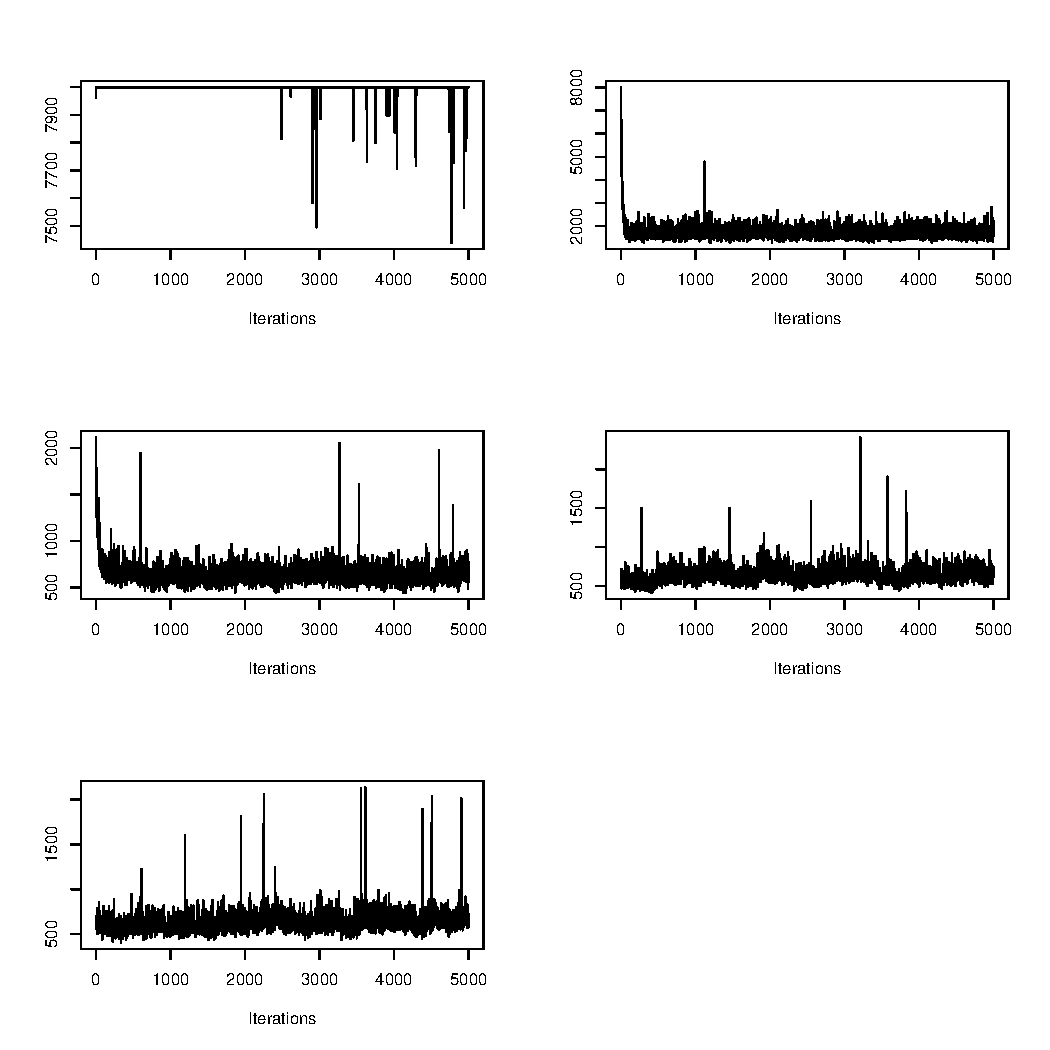
\includegraphics[height=.4\textheight]{5-cycles-max-id}
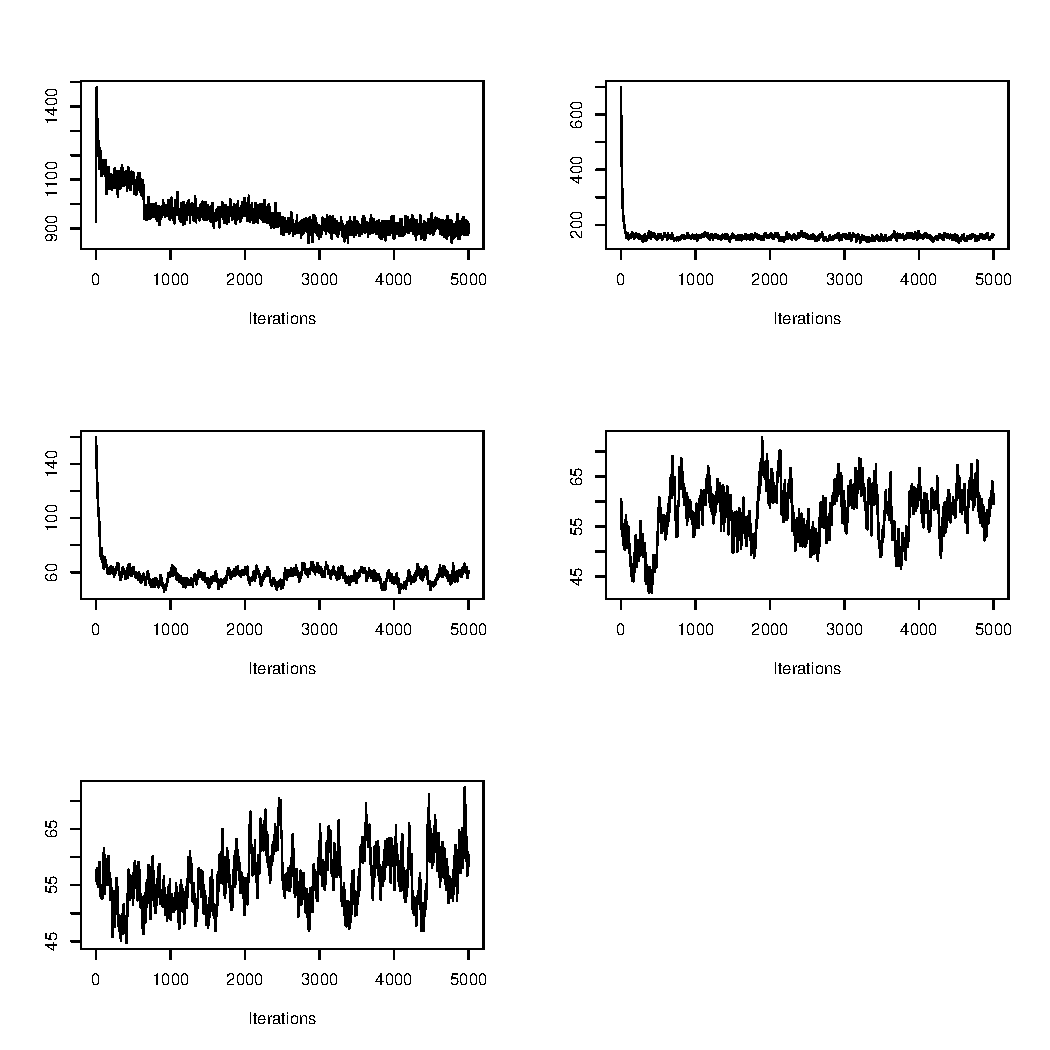
\includegraphics[height=.4\textheight]{5-cycles-alpha}
\caption{Traceplots demonstrating high-level behavior after periodic reordering of cluster ids. Top: 5 series, maximum occupied cluster. Bottom: 5 series, $\alpha$.}
\label{fig:max-id}
\end{figure}


\subsection{Output}
\label{subsec:output}
Because of the dimensionality of the problem is large, memory transfer between the CPU and GPU is slow, and memory on the GPU is limited, it is not feasible to save all of the MCMC samples. Following the approach in \citet{landau2016fully}, we preselect a small number of parameters for which we do save each iteration, but for the rest we first determine which functions of those parameters are of interest and use online algorithms that use running sums to update our estimates of those functions. Without this, we would quickly run out of memory on the GPU or lose a great deal of time due to copying substantial amounts of data each MCMC iteration. The class of estimates we calculate fall into two categories,
\begin{enumerate}
\item expectations of the gene-specific parameters and their squares, i.e. $\op{E} \beta_g,\, \op{E} \beta_g^2,\, \op{E}\sigma_g,\, \op{E}\sigma_g^2$ and 
\item gene-specific posterior probabilities of conjunctions of linear
  inequalities of the elements of $\beta_g$, i.e.,
  $\op{Pr}\left(c_1\beta_g > 0 \land \ldots \land c_t\beta_g > 0\right)$.
\end{enumerate}
Updates of these quantities are embarrasingly parallel across $g$, so are well suited to the GPU. The update in 1) is done elementwise, based on a running sum, and the update in 2) can be decomposed into four tasks, a matrix multiplication to compute $C\beta$, an elementwise evaluation of the sign of the value, a parallel setwise reduction using the minimum to evaluate each conjunction, and finally an update of the estimator (using the same functionality as 1)).

\section{Simulation Study}
The time required by our method will depend both on the raw computational effort, as well as the efficiency of the algorithm. For this reason we choose to use the time per effective sample, which incorporates both of these factors. In particular, we focus on $\alpha$ for simplicity and because it tends to reflect changes in the overall behavior of the Gibbs sampler.

For our experiment, we considered three factors: $G$, the number of genes, $p$, the dimension of $\beta_g$, and $K$, the truncation limit. For each combination of the levels of these three factors we simulated data as follows:

\begin{enumerate}
  \item Let $K_{occ} = \op{floor}(G^{0.5})$. For $k=1 \ldots K_{occ}$, draw $\tilde{\beta}_k \sim \op{N}(0, C),\; \tilde{\sigma^2}_k \sim \op{IG}(1, 1)$, where $C=\op{diag}(3, 3/2^2, \ldots, 3/p^2)$.
  
  \item For $g=1,\ldots G$, draw $\zeta_g \sim \op{Cat}(1/K_{occ},\ldots,1/K_{occ})$. 
  
  \item Let $X = \begin{pmatrix} 1_{4 \times 1} & 0_{1\times(p-1)}\\
                                 1_{4(p-1) \times 1} & I_{(p-1)\times(p-1)} \end{pmatrix}$. Draw $y_{g} \sim \op{N}(X\tilde{\beta}_{\zeta_g}, \tilde{\sigma}^2_{\zeta_g}).$
\end{enumerate}


In this experiment we set $m_\beta = m,\, C_\beta = C,\, a_\sigma^2=1,\, b_\sigma^2=1$, matching the true values, and we set the prior for $\alpha$ as described in section \ref{sec:model}.

Figure \ref{sec-per-mcmc} shows the time per MCMC iteration for each simulation. It appears that the time required grows sublinearly in $G$ and linearly in $K$. We should note that the sample size, $N$, itself has no impact, because the sufficient summary statistics do not scale with $N$.

\section{Example: Paschold maize data}
\citet{paschold} produced an RNA-seq data set for gene expression of root tissue from samples, one sample from each of four young plants representing each of four maize genotypes. The genotypes were two recombinant inbred varieties, B73 and Mo17 and two crosses, B73$\times$Mo17 and Mo17$\times$B73. The plants were at an early stage where phenotypical differences between the genotypes were not yet displayed. A potentially interesting feature that RNA-seq can help address is which genes demonstrate evidence of a difference in expression between two genotypes. At present, we will consider B73 and B73$\times$Mo17.

\subsection{Model}
We let $Y_{gci} = \log \frac{Z_{gci}+1}{C_{ci}}$, where $Z_{gi}$ is the total read count for replicate $i$ of genotype $c$. $C_{ci}$ is a normalizing constant which is used to adjust for differences in the total RNA content in each sample. We estimate the normalizing constants using the trimmed mean of M-values procedure \cite{robinson2010} using \code{edgeR::calcNormFactors()}. The sequencing was done using NextGen sequencing technology across two flow cells, with two replicates of each genotype split across flowcells. This allows us to estimate possible gene specific flow cell effects. Our (abbreviated) design matrix for each gene is then

\begin{equation*}
\begin{blockarray}{rlrrr}
  && \mbox{(Intercept) }\beta_1 & \mbox{(Half-Diff.) }\beta_2 & \mbox{(Flow cell) }\beta_3\\
  \begin{block}{rl(rrr)}
  \mbox{B73}            &\mbox{reps:1,2} & 1 & -1 & 0\\
  \mbox{B73}            &\mbox{reps:3,4} & 1 & -1 & 1\\
  \mbox{B73$\times$Mo17}&\mbox{reps:1,2} & 1 & 1 & 0\\
  \mbox{B73$\times$Mo17}&\mbox{reps:3,4} & 1 & 1 & 1\\
  \end{block}
\end{blockarray}
\label{design}
\end{equation*}

\subsection{Comparison of methods}
In addition to our method, we also fit the data using two other model: a linear mixed-effects model, treating gene-specific parameters as random effects, and all genes independently using least squares. For every method we parameterized the gene-specific mean by an intercept term and a half-difference term -- $\frac{1}{2}(\mbox{B73}\times\mbox{Mo17}-\mbox{B73})$. The independence model, which produces a gene-specific variance estimate borrows no information across genes. The linear mixed-effects model assumes a bivariate normal distribution for all the gene-specific mean parameters. Because the covariance and the mean of this distribution is estimatated from the data, this model does borrow information across genes (since software assumes a zero mean for the random gene effects, we also estimate a fixed effect which corresponds to the unknown mean.) This method assumes homogeneity of the error variance across genes.

\begin{figure}
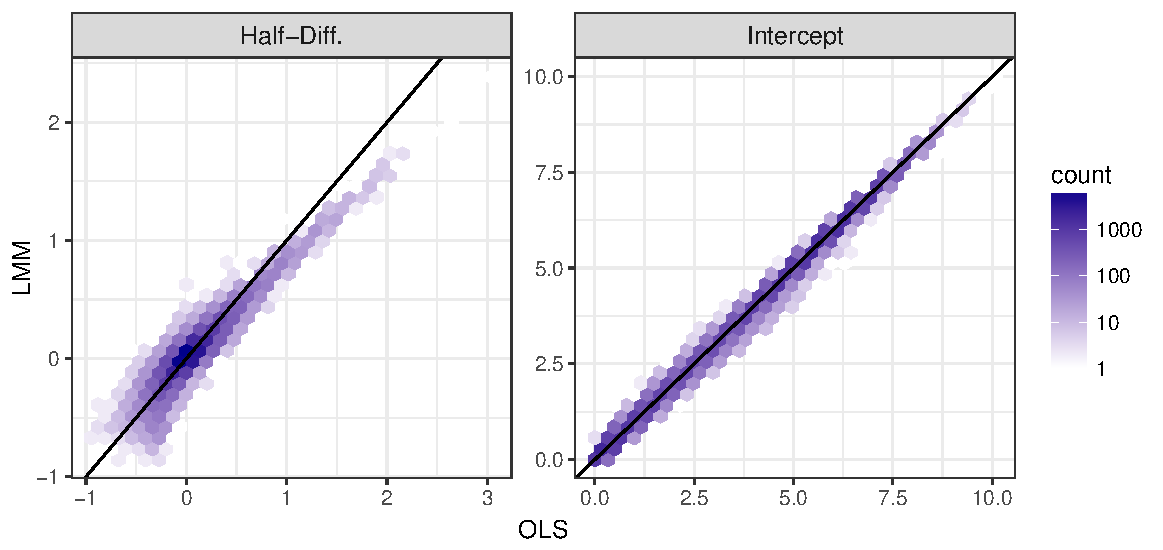
\includegraphics[width=.7\textwidth]{lmm_v_ols.pdf}
\caption{Comparisons of the parameter estimates under each method.}
\label{lmm_v_ols}
\end{figure}
Figure \ref{lmm_v_ols} shows a comparison of the estimates under these two models. While there is agreement about the gene-specific intercepts in the two models, there is noticable shrinkage toward the global mean for the half-difference in the linear mixed-effects model. This can be explained by the long tail of these estimates relative to a normal distribution.

\begin{figure}
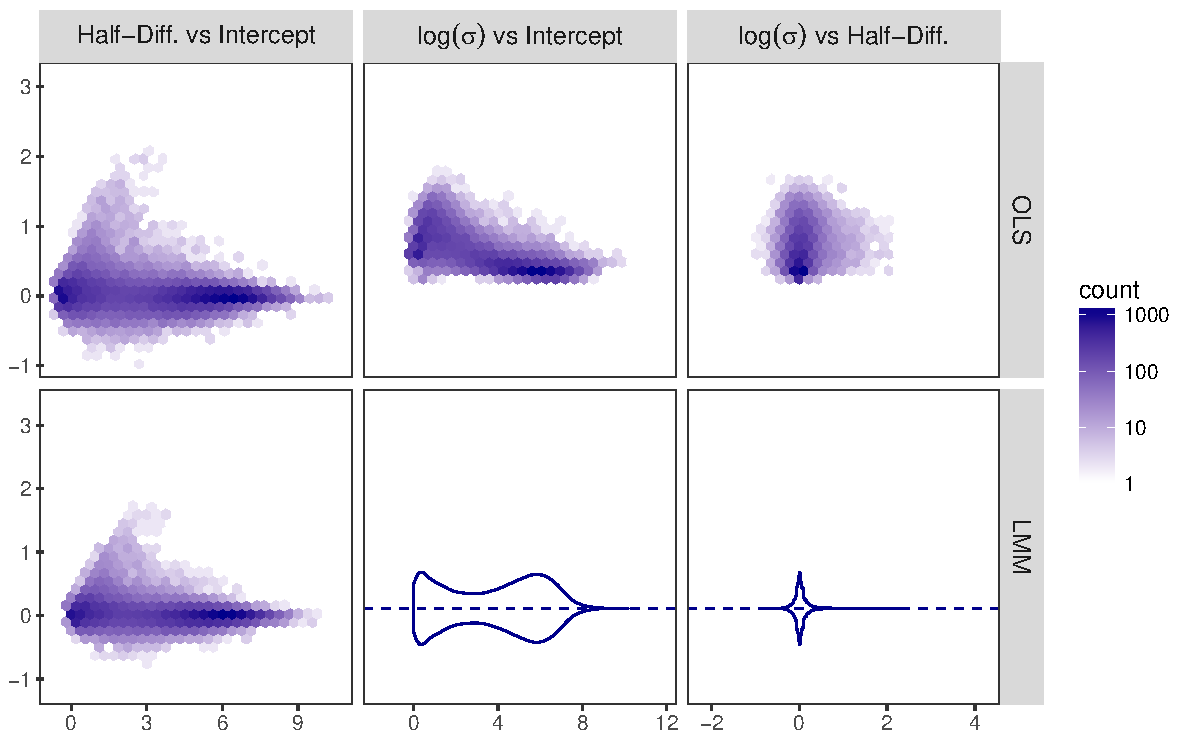
\includegraphics[width=.9\textwidth]{type_v_pairs}
\caption{Bivariate histograms and violin plots describing the joint distribution of estimates obtained from all methods}
\label{type_v_pairs}
\end{figure}

Plotting pairs of parameter estimates obtained from the different methods shows slight differences in the joint distribution of the gene-specific mean parameters for OLS when compared with those obtained by LMM. The most notable difference between the two models being the homogenous variance assumption of LMM. As suggested here, there is a decreasing trend toward lower variability, as a proportion of the mean, as the mean expression increases.


\ref{type_v_pairs}  




Of particular interest was the identification of genes where the mean hybrid expression is higher or lower than that of both parents. For each gene, a reduced version of the design matrix (collapsing identical rows) is
\begin{equation*}
\begin{blockarray}{lcccc}
  & \beta_1 & \beta_2 & \beta_3 & \beta_4\\
  \begin{block}{l(cccc)}
  \mbox{B73} & 1 & 1 & 0 & 0\\
  \mbox{Mo17} & 1 & -1 & 0 & 0\\
  \mbox{B73$\times$Mo17} & 1 & 0 & 1 & 1\\
  \mbox{Mo17$\times$B73} & 1 & 0 & 1 & -1\\
  \end{block}
\end{blockarray}
\label{design}
\end{equation*}

In figure \ref{ggpairs_us}, histograms of the empirical distributions of the OLS estimates are shown. The irregularities seen here contraindicate the use of simple independent parametric models for the underlying parameters. In particular, we note the multimodality of $\beta_1$, the rotated `V' shape of $(\beta_2,\beta_3)$. Despite a large number of genes, we suspect that a misspecification of the model for these parameters will limit the efficacy of borrowing information across genes. We seek to improve the efficacy of borrowing information by relaxing the model to allow Bayesian learning about the underlying distribution of these parameters.
\begin{figure}
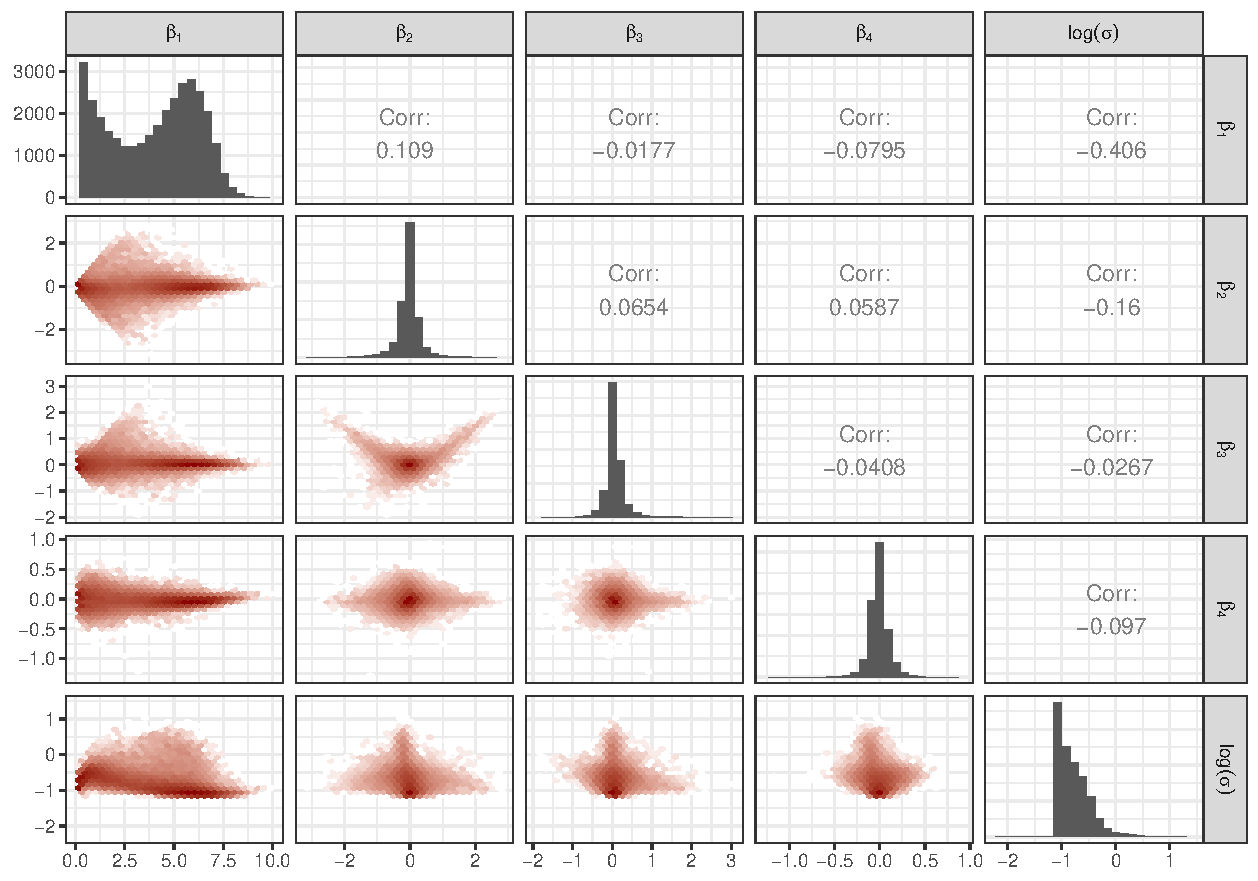
\includegraphics[width=\textwidth]{ggpairs_us}
\caption{Histograms and pairwise histograms of independent OLS
  estimates to for $(\beta_g,\log \sigma_g)$ for all genes in Paschold data set with a non-zero count.}
\label{ggpairs_us}
\end{figure}

Estimates of the posterior means after fitting our model are shown in figure \ref{ggpairs_s}.
\begin{figure}
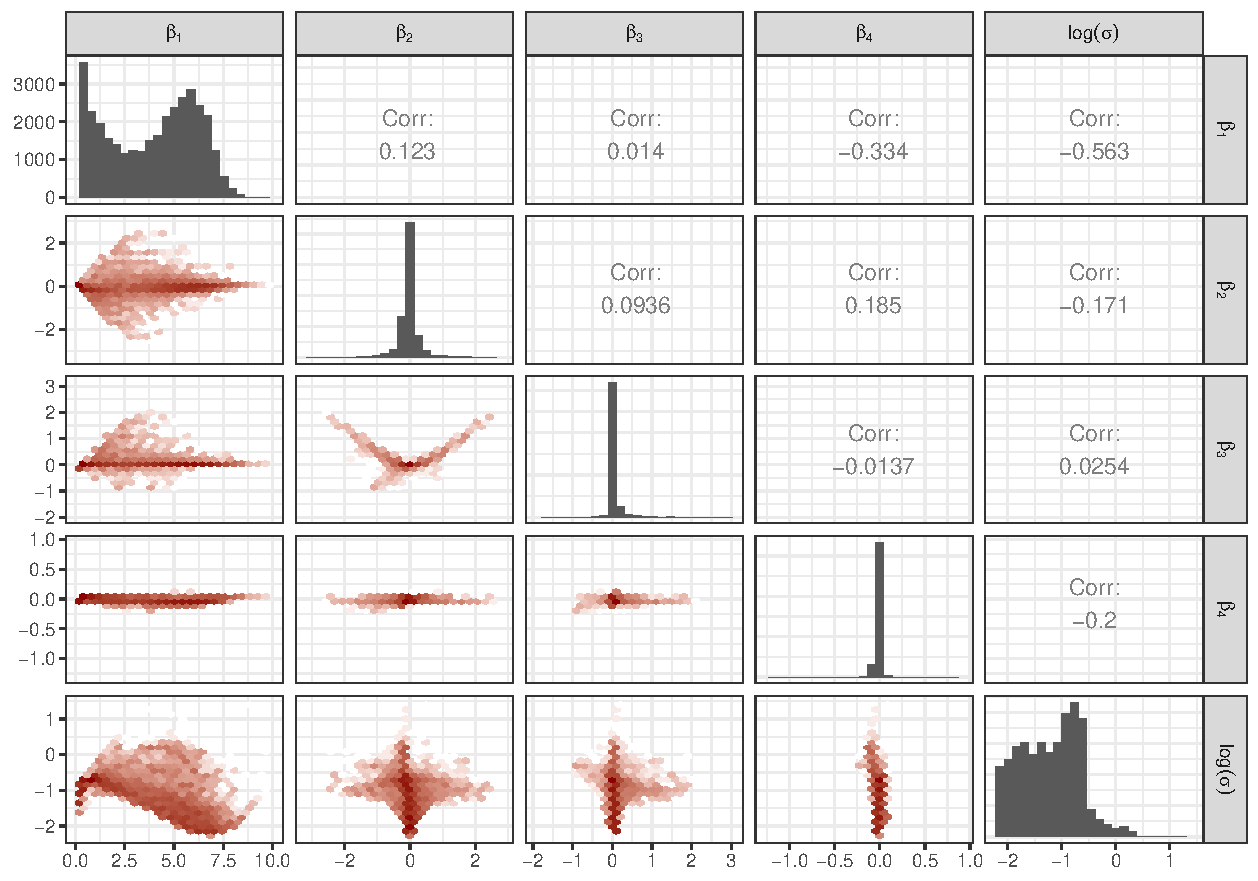
\includegraphics[width=\textwidth]{ggpairs_s}
\caption{Histograms and pairwise histograms of posterior means of
  nonparametric model. Relative to the estimates in Figure
  \ref{ggpairs_us}, there is substantial shrinkage acheived by latent
  clustering.}
\label{ggpairs_s}
\end{figure}

\section{Discussion}
Summarise the contribution of this paper. May want to discuss possible extensions, such as changing the data model, adding label-switching moves, etc.




